\documentclass{beamer}

\usetheme{Darmstadt}
\useinnertheme{circles}
% \setbeamertemplate{items}[triangle]
\usecolortheme{orchid}


\usepackage[utf8]{inputenc}
\usepackage[ngerman]{babel}

\usepackage[scaled]{helvet}
% \renewcommand\familydefault{\rmdefault} % this forces helvetiva for everyting
% \renewcommand{\sfdefault}{phvn} % Sans-Serif font, Helvetica
\renewcommand{\rmdefault}{qpl} % serif font, Tex Gyre Pagella
\renewcommand{\ttdefault}{cmtt} % Typewriter font, Computer Modern Typewriter
\usepackage[T1]{fontenc}

% Better tables
\usepackage{tabularx}
\usepackage{xcolor} % more colors
\usepackage{colortbl} % color cells
\usepackage{booktabs} % \midrule & \toprule & \bottomrule
\usepackage{multirow} % multi-row cells in tables

% Use have more float options
\usepackage{float}
% float figures left/right
\usepackage{wrapfig}

% Multi column layouts
\usepackage{multicol}

% Use graphics
\usepackage{graphicx}

% Better equation environment
\usepackage{amsmath}

% Symbols for most SI units
\usepackage{siunitx}

\usepackage{csquotes}

% be able to include source code listings
\usepackage{listings}
\usepackage{inconsolata}
\definecolor{dkgreen}{rgb}{0,0.5,0}
\definecolor{dkblue}{rgb}{0,0,.6}
\definecolor{dkyellow}{cmyk}{0.2,0,0.8,0.3}
\lstset{
    basicstyle         = \footnotesize{\ttfamily},         % Code font, Examples: \footnotesize, \ttfamily
    breaklines         = true,                           % automatic line breaking only at whitespace
    captionpos         = b,                              % sets the caption-position to bottom
    backgroundcolor    = \color{white},                  % Choose background color
    frame              = tb,                         % A frame around the code
    tabsize            = 4,                              % Default tab size
    captionpos         = b,                              % Caption-position = bottom
    % postbreak          = \mbox{$\hookrightarrow$\space},
    showspaces         = false,                          % Dont make spaces visible
    showtabs           = false,                          % Dont make tabs visible
    inputencoding      = utf8,
    extendedchars      = true,                           % i have some special chars...
    mathescape         = false,                          % i do not like fancy formulas
    escapeinside       = {},                             % i do not like to escape something
    escapechar         = {},                             % so i have no char defined
    texcl              = false,                          % and i do not wanna make fancy comments too..
    numbers            = left,
    language           = php,
    numberstyle        = \ttfamily,
    basicstyle         = \small\ttfamily,
    keywordstyle       = \color{dkblue},
    stringstyle        = \color{red},
    identifierstyle    = \color{black},
    commentstyle       = \color{gray},
    emph               = [1]{php,if,and,or,else,for,if,foreach,as,function,echo,break,continue,switch,case},
    emphstyle          = [1]\color{dkyellow},
    emph               = [2]{public,class,abstract,private,protected,interface,use,trait,namespace,static,this,\$this,extends,implements},
    emphstyle          = [2]\color{dkblue},
    emph               = [3]{int,string,array,mixed,float,double},
    emphstyle          = [4]\color{dkgreen},
}

\usepackage{listingsutf8}

% making diagrams
\usepackage{tikz}
\usetikzlibrary{arrows,automata}
\usetikzlibrary{positioning}
\tikzset{>=latex}


% Bibliography & citing
\usepackage[
	backend=biber,
	style=apa,
	bibstyle=apa,
	citestyle=apa,
	sortlocale=de_DE
	]{biblatex}
\bibliography{Referenzen.bib}
\DeclareLanguageMapping{ngerman}{ngerman-apa}


% Clickable Links to Websites and chapters
\usepackage{hyperref}
% \hypersetup{
%   colorlinks   = true, %Colours links instead of ugly boxes
%   urlcolor     = RoyalPurple, %Colour for external hyperlinks
%   % linkcolor    = Sepia, %Colour of internal links
%   % citecolor   = Sepia %Colour of citations
% }

% shortcut to create refrences
\newcommand*{\fullref}[1]{\hyperref[{#1}]{\ref*{#1}. ``\nameref*{#1}''}}


\usepackage{amssymb}
\usepackage{pifont}



\title % (optional, only for long titles)
{Untersuchung der Performance des Invisible Internet Protocols (I2P)}
\subtitle{Bachelorarbeit}
\author[mkuettel] % (optional, for multiple authors)
{Moritz~Küttel}
\institute[Hochschule Luzern Informatik] % (optional)
{
  Hochschule Luzern Informatik\newline
  \and
  in Zusammenarbeit mit
  \and
  DIVA.EXCHANGE
}
\date[21.4.2021] % (optional)
{Zwischenpräsentation, 21.4.2020}
\subject{Software Engineering; Software Testing; Test automation; Legacy Software; Software Maintenance; Computer Science}




\AtBeginSection[]
{
  \begin{frame}
    \frametitle{Inhaltsverzeichnis}
    \tableofcontents[currentsection]
  \end{frame}
}
\begin{document}

    \begin{frame}
        \maketitle
    \end{frame}

\section{Einleitung und Aufgabenstellung}
    \begin{frame}
        \frametitle{Einleitung}
        \begin{center}
            Der Verein DIVA.EXCHANGE entwickelt einen Softwareprotoypen für eine \textit{vollständig verteilte} Handelsplattform
            \vfill
            Benutzer sollen digitale Werte austauschen können
            \vfill
            \textit{ohne sich zu kennen}
            \vfill
            und
            \vfill
            \textit{ohne gegenseitiges vertrauen}
        \end{center}
    \end{frame}


        % 2mnin + mit inhalsverzeichnis


    \begin{frame}[allowframebreaks]
        \frametitle{DIVA.EXCHANGE Architektur}

        \begin{figure}[thp!]
            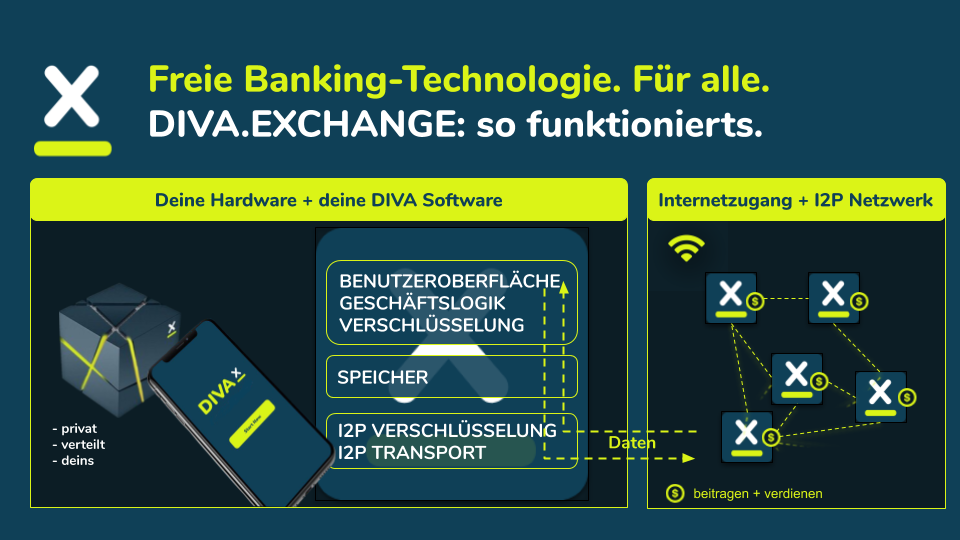
\includegraphics[width=1.0\textwidth]{img/divax-overview.png}
        \end{figure}


        Der Software-Prototyp besteht aus drei Schichten:

        \begin{itemize}
            \item \textbf{Handelsplattform:} Benutzeroberfläche und Geschäftslogik
            \item \textbf{Speicherschicht:} Blockchain, Speichert die Transaktionen
            \item \textbf{Netzwerkschicht:} Basierend auf dem Invisible Internet Protocol (I2P) für verschlüsselte und anonymisierte Kommunikation zwischen den Knoten
        \end{itemize}

        Der Fokus der Arbeit liegt auf der Netzwerkschicht.
    \end{frame}

    \begin{frame}[allowframebreaks]
        \frametitle{Aufgabe}

        \begin{itemize}
            \item \textbf{Problemstellung:} Initiale Tests haben ergeben, das jedoch die Netzwerk-Schicht zu ``langsam'' ist.
                \begin{itemize}
                    \item Roundtrip einer Nachricht im Bereich von 3-8 Sekunden Latenz im öffentlichen I2P-Netzwerk
                \end{itemize}
              \item\textbf{Ziel: }Herausfinden unter welchen Umständen und Rahmenbedingungen kürzere Latenzzeiten erreicht werden können
            \item \textbf{Fragestellung:} Verringert sich die Latenz der Nachrichten je mehr Knoten sich am Netzwerk beteiligen?
            \item \textbf{Vorgehen:} Mittels eines Teststands sollen Latenzmessungen durchgeführt werden, um die Fragestellung empirisch beantworten zu können.
            \item \textbf{Vision:} Könnte dies belegt werden, könnten mehr Leute überzeugt werden einen I2P-Knoten zu betreiben. Dies würde das Netzwerk stärken.
        \end{itemize}

    \end{frame} % 2 + 6 min

    \begin{frame}
        \frametitle{Anforderungen}

        \begin{itemize}
            \item Stand der Technik bezügl. I2P und dem zu erstellenden Teststand erfassen
            \item Das Testnetzwerk soll isoliert sein und abgeschottet vom öffentlichen I2P Netzwerk
            \item Es sollen verschiedene Messungen mit verschiedenen Konfigurationseinstellungen getätigt werden können.
            \item Es soll möglich sein schnell (innerhalb von 2h) eine Messung mit anderer Konfiguration zu starten
            \item Die Anzahl I2Pd-Knoten im Testnetzwerk soll konfigurierbar sein (8-256).
            \item Die Messungen im Teststand sollen reproduzierbar sein
            \item Es soll eine quantitative Auswertung durchgeführt werden.
          \end{itemize}
    \end{frame}

\section{Stand der Technik}
    \begin{frame}
        \frametitle{Das Anonymitätstrilemma}

        \begin{figure}[h]
            \begin{tikzpicture}
              \draw (0,0) node[anchor=north]{hoher Anonymitätsgrad}
                -- (4,0) node[anchor=north]{tiefe Latenzzeiten}
                -- (2,4) node[anchor=south]{wenig Netzwerkbandbreite}
                -- cycle;
            \end{tikzpicture}
        \end{figure}

        Es muss ein passender Kompromiss zwischen diesen Aspekten gefunden werden.

        % Siehe \cite{das_anonymity_2018}
    \end{frame} % 2 + 6 + 1  min

    \begin{frame}
        \frametitle{Invisible Internet Protocol (I2P)}

        \begin{tikzpicture}[remember picture,overlay]
            \node[xshift=-2cm,yshift=-2.5cm] at (current page.north east) {
\includegraphics[scale=0.3]{img/i2plogo.png}};
        \end{tikzpicture}

        \begin{itemize}
            \item Dezentrales, Peer-to-Peer-Netzwerk bestehend aus I2P-Routern/Knoten
            \item Overlay-Netzwerk, ''verstecktes'' Netzwerk innerhalb vom bestehenden IP-Netzwerk
            \item Nachrichtenbasiert (vergleichbar mit IP/UDP)
            \item Mischnetzwerk, Nachrichten können über mehrere Knoten geroutet werden, um Herkunft zu verschleiern
            \item End-to-End Verschlüsselung von Nachrichten
        \end{itemize}

        Wir legen den Fokus auf die C++-Implementation (i2pd) und nicht auf die Java-Implementation (i2p).

    \end{frame} % 4min


\section{Konzept Teststand}

    \begin{frame}[allowframebreaks]
        \frametitle{Konzept}

        \begin{itemize}
            \item \textbf{Reproduzierbarkeit}: Infrastruktur des Teststands als Code, Privates Testnetzwerk
            \item \textbf{Deployment}: Ein Container pro I2P-Router/Knoten
            \item \textbf{Konfigurierbarkeit}: Anzahl Container/Knoten, verschiedene Router-Konfigurationen
            \item \textbf{Isolierung}: Abschotten vom öffentlichen Netzwerk, VM mit Firewallregeln
            \item \textbf{Latenzmessung}: Verschicken von Nachrichten von Knoten an andere. $Latenz = Ankunftszeitpunkt - Sendezeitpunkt$
            \item \textbf{Bootstrapping}: Extra Container welche initialen Netzwerkkoordinaten der Knoten verteilt (reseeder)
        \end{itemize}

        \begin{figure}[ht]
          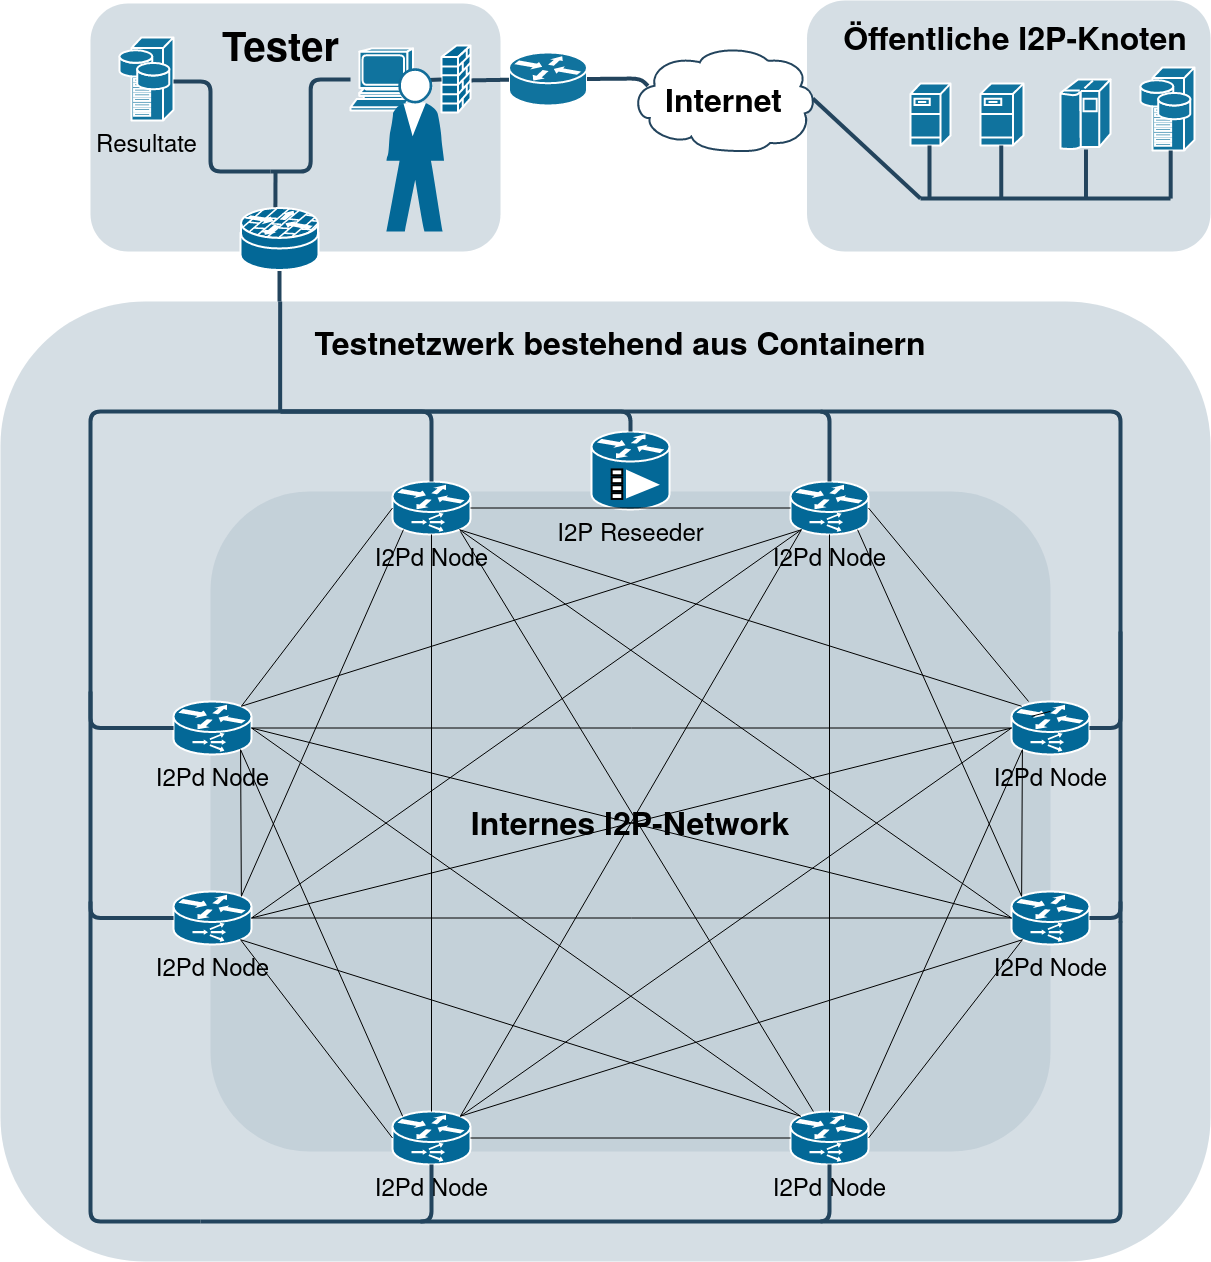
\includegraphics[height=0.8\textheight]{img/i2p-testnetwork.png}
        \end{figure}
    \end{frame}

\section{Projektverlauf}

    \begin{frame}
        \frametitle{Projektverlauf}

        \begin{itemize}
            \item 1. Ansatz NixOS/NSpawn Container
                \begin{itemize}
                    \item Erst Probleme mit der Netzwerkkonfiguration
                    \item Probleme mit Docker-Kompatibilität
                    \item Skaliert nicht auf mehr als ein paar dutzend Container. Zu viel RAM benötigt lediglich zum Berechnen der verschiedenen Container-Konfigurationen.
                \end{itemize}
            \item Deshalb umgestiegen auf \lstinline|docker-compose|-Ansatz
                \begin{itemize}
                    \item 256 \lstinline|i2pd|-Container konnten erstellt werden
                    \item Wiederverwendung bestehender Docker-Container
                    \item Anfangs triviale Netzwerkkonfiguration, aber ich stosse damit an Grenzen.
                \end{itemize}
        \end{itemize}
    \end{frame}


    \begin{frame}
        \frametitle{Jetziger Stand}

        Folgendes im Teststand ist implementiert:

        \begin{itemize}
            \item Konfigurierbare Anzahl-Knoten
            \item Isolierung vom öffentlichen Netzwerk
            \item Bootstrapping / Reseeding erfolgreich
            \item Angefangen mit TCP-Server zum Messen der Latenz
            \item Probleme mit der Netzwerkkonfiguration
        \end{itemize}

        Das Projekt ist im Verzug, der Teststand sollte bereits Ende letzte Woche fertig sein.
    \end{frame}


\section{Abschluss}

    \begin{frame}
        \frametitle{Weiteres Vorgehen}

        \begin{itemize}
            \item Lösen der Netzwerkkonfigurationsprobleme
            \item Fertigstellung des TCP-Servers zur Latenzmessung
            \item Verschicken von Nachrichten und Latenzmessung
            \item Durchführen von Messungen mit verschiedenen Konfigurationen
            \item Auswertung und Vergleich der Messungen
        \end{itemize}
    \end{frame}

    \begin{frame}
        \frametitle{Abschluss}

        Danke für Ihre Aufmerksamkeit.
        \vfill
        Zeit für Fragen.
    \end{frame}


    \bgroup
    \setbeamercolor{background canvas}{bg=black}
    \begin{frame}[plain]{}
    \end{frame}
    \egroup

    \begin{frame}
        \frametitle{I2P Konzepte und Begrifflichkeiten}

        \begin{itemize}
            \item \textbf{Router-Info} Beinhaltet u.a. Public-Keys und Netzwerkkoordinaten eines I2P-Routers
            \item \textbf{Network Database:} kurz NetDb. Eine DHT wo jeder Knoten Informationen über seine Peers (u.a. Router-Infos) ablegt.
            \item \textbf{Reseeder} Benötigt zum Boostrappen (erstellen eines I2P-Netzwerks) und wenn ein I2P-Router einem Netzwerkbeitritt. Liefert Router-Infos aus.
            \item \textbf{Tunnel} Eine Verbindung über (normalerweise) mehrere Knoten. Tunneltypen:
                \begin{itemize}
                \item \textbf{Inbound:} Eingehende Verbindung
                \item \textbf{Outbound:} Ausgehende Verbindung
                \item \textbf{Exploratory:} Werden verwendet zum Aufbauen von Tunnels
                \item \textbf{Client/Server:} Gateway der in und aus dem I2P-Overlay Netzwerk führen
                \end{itemize}
        \end{itemize}
    \end{frame} % 5 min


    \begin{frame}[allowframebreaks]
        \frametitle{Routing im I2P-Netzwerk}

        \begin{figure}[t]
            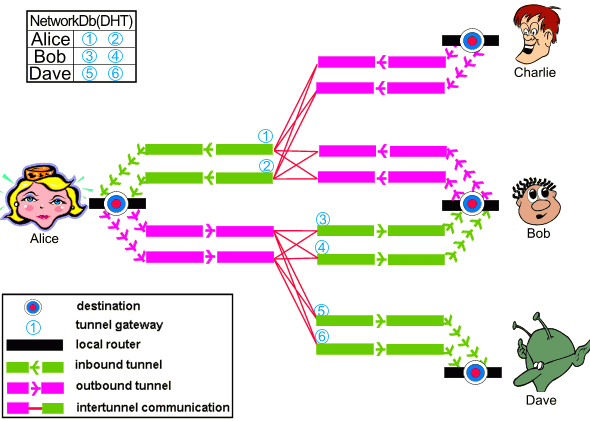
\includegraphics[height=0.69\textheight]{img/i2prouting.png}
            \caption{Garlic-Routing (vgl. \url{https://geti2p.net/de/docs/how/intro})}
        \end{figure}

        Wichtiges:

        \begin{itemize}
            \item Dieser Routing-Mechanismus (Garlic-Routing) ist zur Anonymisierung und Verschlüsselung von Nachrichten
            \item Je länger die Tunnels desto grösser die Latenz, da mehr Hops/I2P-Router sind darin verwickelt.
            \item Jeder Knoten bestimmt die Länge seiner Tunnels selbst
            \item Somit auch den Anonymisierungsgrad und die Latenz
        \end{itemize}

    \end{frame}


    \begin{frame}
        \frametitle{Projektmanagement}

        KanBan wird benutzt als Projektmangament Methode

        \begin{itemize}
            \item Iterativ
            \item Pull-Prinzip
            \item Nur 1 Task auf einmal bearbeiten
            \item Projektboard mit drei spalten (Todo, Doing, Done)
        \end{itemize}
    \end{frame} % 6min


    \begin{frame}
        \frametitle{Wochentagplan}

        \begin{figure}[t]
            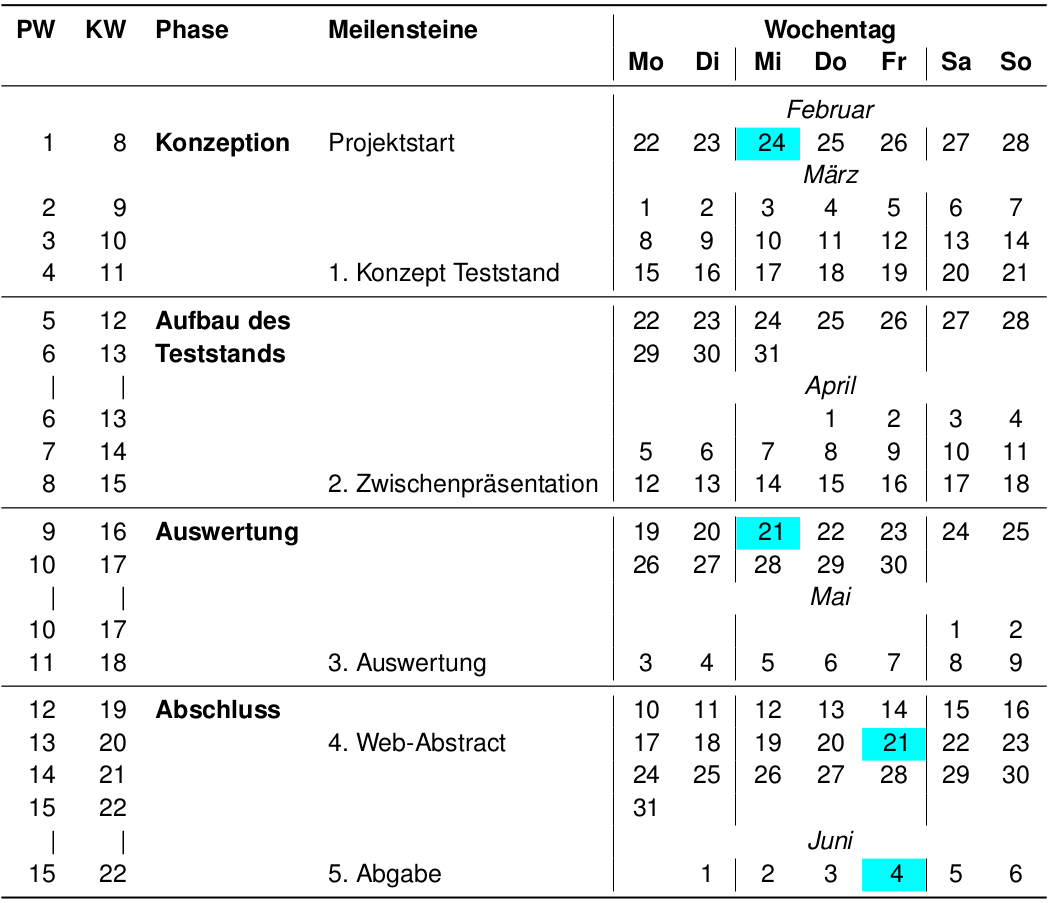
\includegraphics[height=0.8\textheight]{img/wochentagplan.png}
        \end{figure}

    \end{frame} % 6min


    \begin{frame}
        \frametitle{Methode Teststand}

        \begin{itemize}
            \item Qualitative Analyse mit Laborexperiment (E.g. Teststand)
            \item Aufbau des Teststands ist jedoch ein Prototyping Verfahren
        \end{itemize}
    \end{frame} % 6min

\end{document}

% * Project Management methodology (meetings requyirements)
% * Let them know what's happening more
% * Evaluation State Of The Art (e.g. wieso docker / PHPUnit)
%   * how to determine what's state of the art?
%   * provide explanations for why this was chosen
%   * add references
% * mod order first cirtical/complex
%
% Schlusspräsentation:
%
% * Bisher erzaähltes muss nicht erwähnt werden
% * Bezug nehmen auf die Aufgabenstellung/Fragestellung (alle wesentlichen Aspekte des Themenkontexts berücksichtigen)
% * Entscheidungen Nachvollziehbar darlegen
% * Konkret werden mit einem Beispiel
% * Konkret wreden mit Projektmanagement/Engineering
% * Highlights erklären und aufzeigen
